\chapter{Platform Description}

\begin{FraseCelebre}
  \begin{Frase}
    The needs of the many outweigh the needs of the few
  \end{Frase}
  \begin{Fuente}
    Spock - The Wrath of Khan
  \end{Fuente}
\end{FraseCelebre}


We propose a blockchain-enabled decentralized publication system for open
science. It consists of three main components that decentralize and try to
improve three different aspects related to scientific publication:

1) Peer review governance communication is traditionally centralized and
controlled by editors and publishers. Our proposal opens and decentralizes these
communications making the process more transparent.

2) Peer reviewer quality and reliability information is difficult to
predict~\cite{callaham_relationship_2007}, and it is usually hold private by
publishers and journals. The system proposes to open this information through a
decentralized reputation network of peer reviewers over a blockchain.

3) Scientific papers are traditionally obtained or bought from a centralized
publisher. We propose a decentralized network to distribute academic works and
promote free access to science.

These ideas are further discussed in the following sections.

% \section{Decentralized publication system for open science}

% We propose a blockchain-enabled decentralized publication system for open
% science. It consist of three components that decentralizes three different
% aspects of science publication.

% 1) Peer review governance communication is traditionally centralized and
% controlled by editors and publisher. Subsection \ref{workflow} further explore
% the opening and decentralization of this communication with blockchain
% technology.

% 2) Peer reviewer quality and reliability information is difficult to
% predict~\cite{callaham_relationship_2007}, and is usually hold private by
% publishers and journals. The system propose to distribute and open this
% information though a decentralized reputation network of peer reviewers over
% blockchain. Subsection \ref{reputation} further explore this proposal.

% 3) Open access papers are traditionally obtained from a centralized publisher
% infrastructure. Subsection \ref{distributedOA} explores the decentralization
% of this infrastructure.

\subsection{Transparent Peer Review Governance}
\label{workflow}

The system provides a platform for the peer review process communication, from
paper submission to paper acceptance or rejection. It registers all the
interactions into a blockchain based distributed
ledger. % and provides open access to all relevant content, from the different versions of the paper to the submitted reviews.

The interaction diagram of the system (Figure \ref{InteractionDiagram})
describes the interactions of the supported peer review governance. Following,
this interactions and their implementation are described.

  \begin{figure}[!th]
    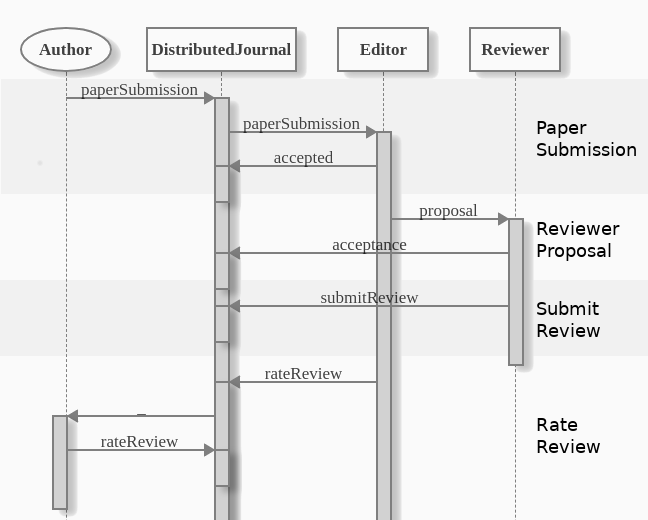
\includegraphics[width=1\linewidth]{Uml.png} \centering\caption{Sequence
      diagram of platform interaction}
    \label{InteractionDiagram}
  \end{figure}

  \begin{LaTeXdescription}
  \item[Paper submission] A paper submission is registered by submitting the
    IPFS address of the paper to an Ethereum contract. Then, the Ethereum sender
    address is recorded as the corresponding author, and the submission is
    timestamped in the blockchain.

  \item[Reviewer proposal] A journal editor may invite a peer reviewer to review
    a specific paper. The transaction will record the Ethereum address of the
    reviewer and optionally, a deadline to submit the review.

  \item[Reviewer acceptance/rejection] An invited reviewer may accept or reject
    the review of a paper. The response will be recorded into the blockchain.

  \item[Submit review] A reviewer should make a transaction to deliver the
    review. The transaction will record the acceptance/rejection and the IPFS
    address of the detailed review.

  \item[Rate review] A novelty of the system further discussed in Section
    \ref{reputation} is the rating system for reviews. The transaction will
    record the sender address and the rating as well as the rated review and
    reviewer addresses.
  \end{LaTeXdescription}

  \subsection{The Peer Review Reputation network}
  \label{reputation}

  The system proposes the use of a peer review reputation network were the
  quality of peer reviews is rated by the authors, editors and reviewers of the
  system. The work extends traditional peer review governance with the
  possibility of rating the reviews, building a reputation system for
  reviewers~\cite{resnick2000reputation}. Reviewers get rewarded for worthy,
  fair, an timely reviews, or penalized otherwise.

  This network of peer reviewers would enable a better reviewer selection, a
  fair recognition of reviewers work and a protection against unfair reviews for
  authors. However, it could also rise privacy concerns for both reviewers and
  raters~\cite{van1999effect,schaub2016trustless}. We consider these privacy
  issues in section \ref{privacy}.

  % With this network of rated peer reviews, different metrics of the peer
  % reviewers can be provided by the system. Journals can benefit from this
  % network by searching for well rated reviewers that respond on time, authors
  % can expect shorter review time and forget about unaccountable bad reviews
  % and reviewers can get their work publicly recognized. This approach can
  % suppose a privacy problem for both reviewers and raters. We contemplate
  % these problems and how to solve them in section \ref{PrivacyReviewRating}.

  \subsection{Distributed Open Access infrastructure}
  \label{distributedOA}
  % \commant{Copied from PEERE Paper.TODO rewrite}
  Open Access focuses in the free access to scientific knowledge. While
  publishers provide free of charge their Open Access content, their control of
  the science dissemination infrastructure allows them to impose certain rules,
  such as charging authors unreasonable fees to offer their work as Open
  Access~\cite{solomon2012study} (Gold Open Access) or the temporal embargo and
  restrictions on the dissemination of the final version (Green Open
  access)~\cite{bjork2014anatomy}, among others.

  The system proposes a decentralized infrastructure for science publication.
  Academic documents - from first drafts to final versions, including peer
  reviews- are shared in IPFS, an open P2P
  network~\cite{benet_ipfs-content_2014}. Thus, the system inherently grants
  Open Access by the design of its distributed infrastructure and circumvents
  the publishers dominant role.

  \section{Privacy Settings of Open Peer Review and Rating}
  \label{privacy}
  Anonymity of reviewers and authors in peer reviews is traditionally used to
  improve the fairness of the process. Thanks to single blind reviews, anonymous
  reviewers can honestly critic a paper without fearing the reactions of the
  authors. Double blind reviews also allow to reduce the impact of personal
  biases. Finally, open review models propose that both authors and reviewers
  know each other. These different privacy settings are shown in the left part
  of Figure \ref{PrivacyReviewRating}.

\begin{figure}[!th]
  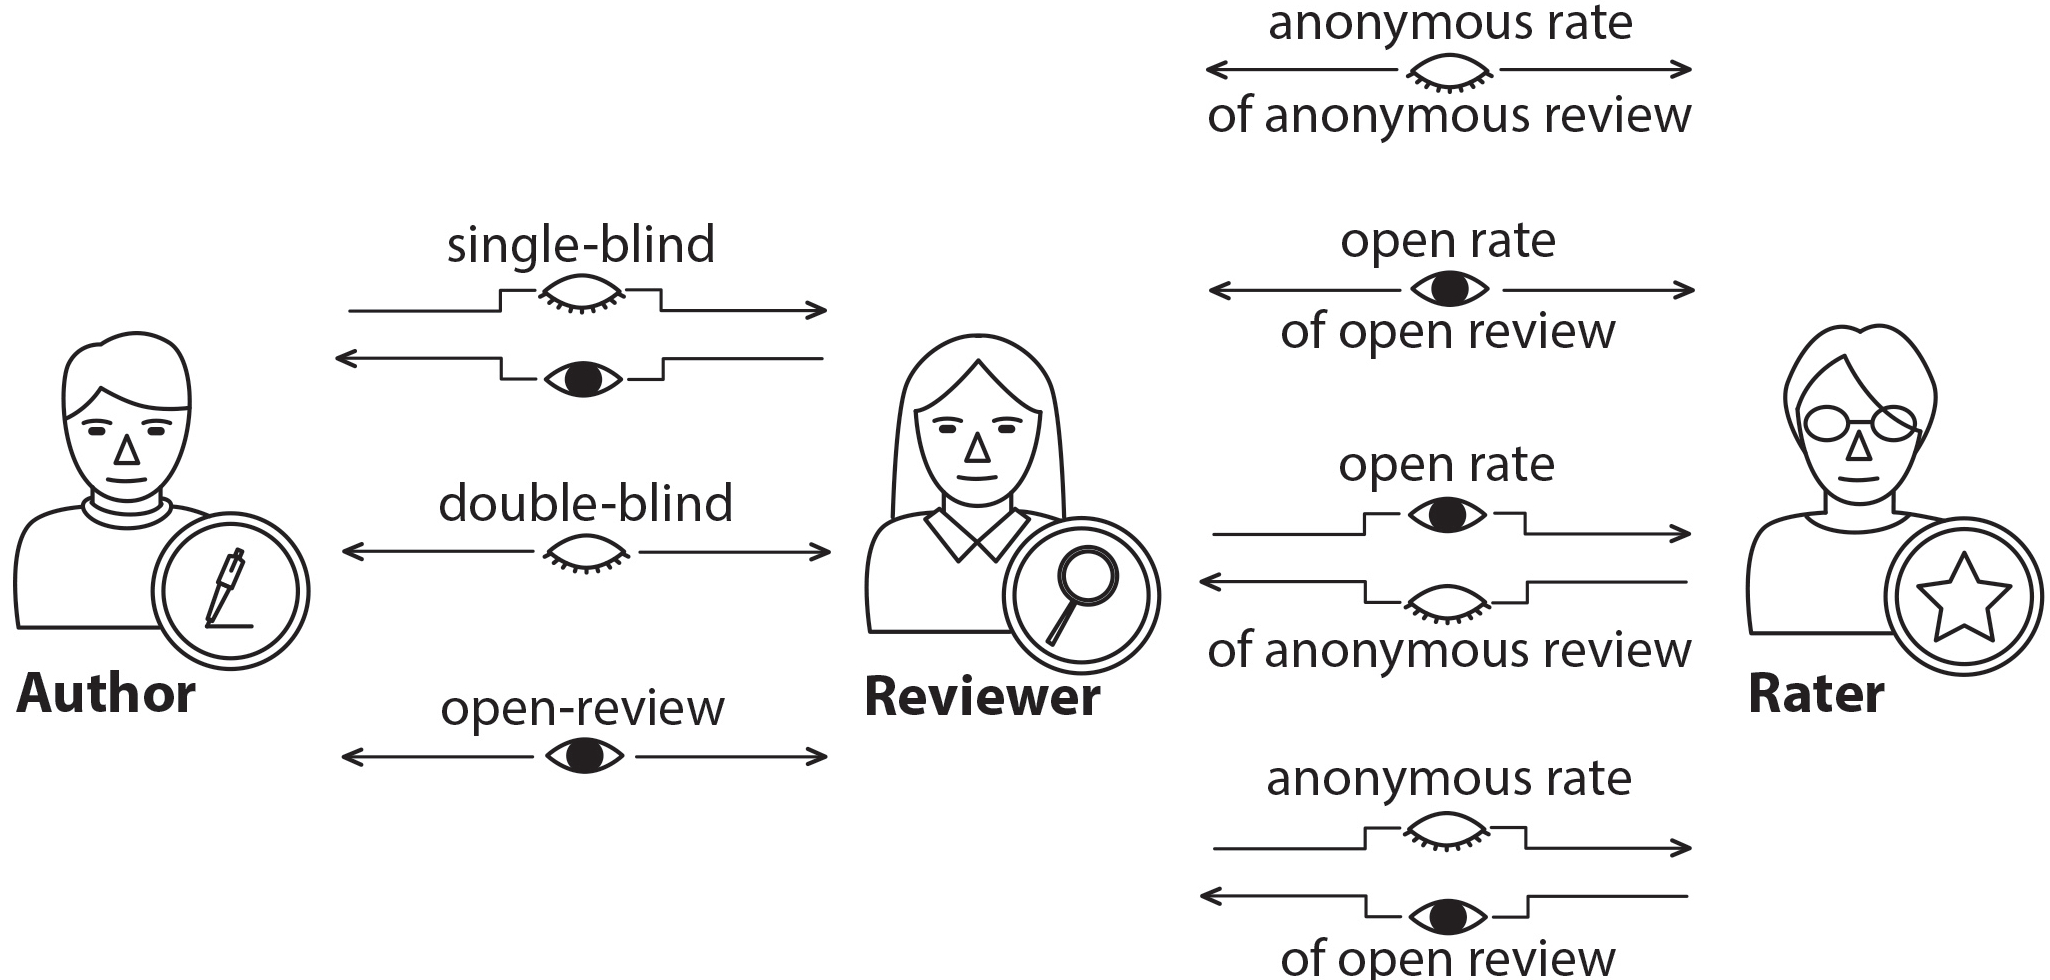
\includegraphics[width=\columnwidth]{privacyReviewRating.jpg}
  \centering \caption{Review and Rating privacy models}
  \label{PrivacyReviewRating}
\end{figure}

Note, however, that the anonymity of the reviewers can be also abused. Unfair
and low quality reviews are not discouraged by the system due to the lack of
consequences. In order to alleviate this problem, our system proposes the
construction of a reputation network of peer reviewers so that reviewers are
awarded or criticized according to their work. This reputation network can also
adopt different privacy settings, allowing both anonymous and signed ratings of
either signed or anonymous reviews as depicted on the right side of Figure
\ref{PrivacyReviewRating}.

The implementation of these different privacy settings in a blockchain requires
different approaches. The question of whether we can keep the benefits of blind
review while providing accountability and recognition to reviewers deserves
special consideration. Next, we discuss the different privacy models for review
and privacy settings.

% Anonymity of reviewers and authors in the peer review process is a simple tool
% traditionally used to improve the fairness of the process. Thanks to single
% blind reviews, anonymous reviewers could honestly critic a paper without
% fearing authors reactions. Double blind reviews allow to reduce the impact of
% biases in the review. Open reviews model however propose that both authors and
% reviewers are known. Left part of Figure \ref{PrivacyReviewRating} illustrate
% these different privacy settings of peer
% review. %\commant{Mañana por la mañana tenemos una versión profesional del diagrama}.

% As already discussed, the anonymity of the reviewers can also be abused.
% Unfair or low quality reviews were not discouraged by the system due to the
% lack of consequences.

% The system propose the construction of a reputation network of peer reviewers.
% This reputation network can also adopt different privacy settings, allowing
% both anonymous and signed ratings of either signed or anonymous reviews as
% depicted in the right side of Figure \ref{PrivacyReviewRating}.

% Each of the anonymity options of the system requires different solutions,
% which are discussed bellow. The question of whether we can keep the benefits
% of blind review while providing accountability and recognition to reviews
% deserves special consideration.

\subsection*{Blind peer review}
Blind review is the protection of the identity of reviewers in the peer review
process. In a blockchain, this protection could be easily achieved by using
single-use addresses previously agreed with the editor.

\subsection*{Double blinded peer review}
A double blinded review is a blind review that additionally protects the authors
identity to prevent social bias~\cite{lee2013bias}~\cite{budden2008double}.
Authors could protect their identities prior to publication by providing a
single-use public address on submission. Later they can reveal their real
identity since they are the only ones with access to that address.

\subsection*{Open peer review}
Open evaluation proposes the de-anonymization of all the parties involved in the
peer review process~\cite{ford2013defining}. While studies found effect on the
percentage of reviewers declining to review~\cite{van1999effect} other
implications remain open to debate~\cite{groves2010open}.

% \subsection*{Blind peer review}
% Blind review is the protection of the identity of reviewers in the peer review
% process. In a blockchain, this protection could be easily achieved by using
% single use addresses or passwords agreed with the editor.

% \subsection*{Double blinded peer review}
% A double blinded review is a blind review that additionally protects the
% authors identity to prevent social
% bias~\cite{lee2013bias}~\cite{budden2008double}. Authors could protect their
% identities prior to publication by providing a single use public key from
% which later they sign their real identity or signing the paper with the hash
% of their names followed by a random constant, revealing the constant after
% acceptance.

% \subsection*{Open peer review}
% Open evaluation proposes the opening and deanonymization of peer
% review~\cite{ford2013defining}. While studies found effect on the percentage
% of reviewers declining to review~\cite{van1999effect} other implications
% remain open to debate~\cite{groves2010open}.

% Signed reviews are easy to implement by maintaining a public identity for the
% reviewer.

\subsection*{Open Rating}

Similarly to open reviews, open ratings are easy to implement by maintaining a
public identity for the raters.

\subsection{Anonymous Rating}

Protecting the identity of raters is interesting in several reputation systems.
We can support this anonymity feature using \emph{blinded tokens}
~\cite{schaub2016trustless} that grant permission to rate without revealing the
identity of the rater. People authorized to rate a review, such as authors,
editors and other reviewers involved in the process, may each get one of these
tokens.

\subsection*{Rating anonymous reviews}

In a system that support voluntary signing of reviews, unsigned reviews would
not affect the reviewers reputation unless they acknowledge their authorship.
Thus, reviewers may only reveal their identities for well rated reviews,
reducing the desired accountability for poor quality, unfair or late reviews.

A system allowing anonymous, yet accountable, reputation system for peer
reviewing is therefore of great interest. Following, we discuss the feasibility
of adopting different anonymity approaches to realize this system.

\emph{Collateral models} are widely used in blockchain technology to ensure that
an actor assumes negative consequences of an interaction in order to avoid the
greater consequence of loosing the collateral. A similar strategy can be used
for the anonymous reputation network. If a reputation collateral is requested
from the reviewers, they would be encouraged to claim even negative ratings.
This model can be combined with anonymity measures to ensure accountable yet
anonymous, peer reviews.

\emph{Coin mixing} protocols are designed to obfuscate the relation between
senders and receivers of Bitcoin payments by mixing in a single transaction many
senders and receivers ~\cite{meiklejohn2015privacy}. We can not directly apply
this approach to rate reviews since the receiver identity is known. However it
can be used in collaboration with other techniques discussed below.

\emph{Reusable payment codes} enable the possibility of using a large amount of
addresses to receive a payment ~\cite{harrigan2016unreasonable,
  ranvierReusable}. Reviewers may share one of this addresses with each of the
actors with permission to rate and then collect the reputation probably using an
anonymity layer such as coin mixing. Using a collateral model would encourage
the acceptance of bad ratings.

\emph{ZK-Snarks} are a cryptographic tool enabling to prove a statement without
revealing anything else than the statement is in fact true (Zero-Knowledge Proof
of Knowledge) ~\cite{blum1988non,bitansky2013succinct}. They also provide this
property in a succinct and non-interactive fashion (i.e. using a relatively
small proof and not requiring further communication between prover and
verifier). Zcash uses this technology to build an anonymous
cryptocurrency~\cite{sasson2014zerocash}. A similar approach could be used to
manage anonymous ratings. A reviewer could also receive the rating of a review
she did without revealing from which review or which rating the reputation
comes. As before, a collateral model can be used to encourage the acceptance of
low ratings.

%%%
%%% Local Variables:
%%% mode: latex
%%% TeX-master: "../Tesis.tex"
%%% End:
